\section{Experiments}
\label{sec:application}

We use the twenty-subject cohort of Sec.~\ref{sec:data} to settle the question
Sec.~\ref{sec:intro} left open: how far standard video understanding gets on
automated rodent seizure detection and severity grading, and where it breaks. This is an applications-track study: we benchmark
existing architectures under a controlled protocol; we do not propose a new
algorithm.

\noindent\textbf{Setup.}
Unless noted, the video model is an R(2+1)D-18
backbone~\cite{tran2018r2plus1d} pretrained on Kinetics-400~\cite{kay2017kinetics}
and fine-tuned on 16-frame $112\times112$ clips. As a matched EEG reference we
train a GRU on the same cohort and split, echoing
Ganguly~\etal~\cite{ganguly2025}, and later broaden this to seven EEG models
(Table~\ref{tab:eegarch}). Splits are session-disjoint to prevent clip leakage,
with the split seed shared between modalities so the two are directly comparable;
we report macro-averaged metrics with per-subject breakdowns and inverse-frequency
class weighting throughout (Sec.~\ref{sec:problem}). Our headline comparison
(Table~\ref{tab:results}) contrasts video and the EEG GRU across all three task
granularities. Single runs use seed 42 throughout; Table~\ref{tab:results} also
reports macro-F1 as mean\,$\pm$\,std over five seeds, which bounds how much of any
margin below can be attributed to initialization. App.~\ref{sec:arch} describes every model in more detail, video backbones in App.~\ref{sec:arch:video} and EEG models in App.~\ref{sec:arch:eeg}, together with the training recipe they all share (App.~\ref{sec:arch:train}).

% fig:detexample now lives in the supplement (App. C, sec:dataextra:stages),
% alongside the per-stage filmstrips; it is cited from here and from Sec. 4.

\subsection{What model and input capacity is sufficient?}
\label{sec:rq1}

Before comparing modalities we ask what it takes to read seizure behavior from video
at all. Four questions matter: how much signal the medium carries, how much network is needed to extract it, how much of each clip must be sampled, and how much of the result comes from shortcuts. We answer each in turn, holding the protocol of Sec.~\ref{sec:problem} fixed and varying one factor at a time.

\noindent\textbf{Step 1: video carries a strong recognition signal.}
Fine-tuned on 16-frame $112\times112$ clips, R(2+1)D-18 reaches $0.968\pm0.002$ macro-F1
and $0.993\pm0.001$ AUROC at detection over five seeds (Table~\ref{tab:results}). The clip construction makes this
a test of behavior rather than of scene: every seizure clip is paired with a
non-seizure clip from the \emph{same} animal and the \emph{same} session, so camera,
cage and lighting are identical within a pair and cannot by themselves separate the
two (App.~\ref{sec:dataextra:stages}, Fig.~\ref{fig:detexample}). The result holds animal by animal. Per-subject detection macro-F1 exceeds 0.90 on the well-represented subjects, 0.974 on R1 and 0.906 on R7, and degrades gracefully on the near-silent ones, where only a handful of validation clips exist. Behavior alone therefore supports near-ceiling detection on this cohort, echoing the false-positive reductions video brought to human vEpiNet~\cite{vepinet2024}. Sec.~\ref{sec:crossmodal} takes up how it compares against an electrode-based reference.

\begin{table}[t]
\centering
\caption{Application results on the pooled twenty-subject cohort (session-disjoint). Video
(R(2+1)D-18) \vs\ a matched EEG GRU. Precision, recall and F1 are macro-averaged;
AUROC is binary at detection and macro one-vs-rest at grading; MCC is the
multiclass Matthews correlation coefficient, computed from the full confusion matrix
and so weighted towards the frequent classes that macro-F1 down-weights. Every entry is mean\,$\pm$\,std over five
seeds, so each comparison can be read against its own initialization noise;
Tables~\ref{tab:vidarch}, \ref{tab:eegarch} and~\ref{tab:frames} instead report
single seed-42 runs. EEG clip scores use logmean window pooling throughout, selected
by the sweep of App.~\ref{sec:eegsweep}. EEG edges video at detection on all five
metrics---a 0.006 macro-F1 margin that is small but consistent (Welch
$p{=}0.003$)---and video leads at both grading granularities. The one crossover is
5-class AUROC, where EEG ranks clips better (0.945 \vs\ 0.939) while scoring far
worse once those rankings are turned into decisions (macro-F1 0.560 \vs\ 0.657).
Best in \textbf{bold}, second-best \underline{underlined}.}
\label{tab:results}
\setlength{\tabcolsep}{4pt}
\renewcommand{\arraystretch}{1.2}
\resizebox{\columnwidth}{!}{%
\begin{tabular}{@{}l l c c c c c@{}}
\toprule
\textbf{Task} & \textbf{Modality} & \textbf{Prec.} & \textbf{Rec.} & \textbf{F1} & \textbf{AUROC} & \textbf{MCC} \\
\midrule
\multirow{2}{*}{2-class (detection)} & Video & \underline{0.968}\,{\scriptsize$\pm$0.002} & \underline{0.968}\,{\scriptsize$\pm$0.002} & \underline{0.968}\,{\scriptsize$\pm$0.002} & \underline{0.993}\,{\scriptsize$\pm$0.001} & \underline{0.936}\,{\scriptsize$\pm$0.004} \\
                                     & EEG   & \textbf{0.975}\,{\scriptsize$\pm$0.002} & \textbf{0.974}\,{\scriptsize$\pm$0.003} & \textbf{0.974}\,{\scriptsize$\pm$0.003} & \textbf{0.996}\,{\scriptsize$\pm$0.001} & \textbf{0.949}\,{\scriptsize$\pm$0.005} \\
\midrule
\multirow{2}{*}{3-class (severity)}  & Video & \textbf{0.775}\,{\scriptsize$\pm$0.016} & \textbf{0.788}\,{\scriptsize$\pm$0.009} & \textbf{0.780}\,{\scriptsize$\pm$0.007} & \textbf{0.964}\,{\scriptsize$\pm$0.003} & \textbf{0.853}\,{\scriptsize$\pm$0.010} \\
                                     & EEG   & \underline{0.744}\,{\scriptsize$\pm$0.014} & \underline{0.764}\,{\scriptsize$\pm$0.013} & \underline{0.750}\,{\scriptsize$\pm$0.010} & \underline{0.956}\,{\scriptsize$\pm$0.002} & \underline{0.823}\,{\scriptsize$\pm$0.014} \\
\midrule
\multirow{2}{*}{5-class (severity)}  & Video & \textbf{0.689}\,{\scriptsize$\pm$0.024} & \textbf{0.643}\,{\scriptsize$\pm$0.006} & \textbf{0.657}\,{\scriptsize$\pm$0.009} & \underline{0.939}\,{\scriptsize$\pm$0.004} & \textbf{0.831}\,{\scriptsize$\pm$0.006} \\
                                     & EEG   & \underline{0.556}\,{\scriptsize$\pm$0.040} & \underline{0.635}\,{\scriptsize$\pm$0.035} & \underline{0.560}\,{\scriptsize$\pm$0.005} & \textbf{0.941}\,{\scriptsize$\pm$0.003} & \underline{0.728}\,{\scriptsize$\pm$0.032} \\
\bottomrule
\end{tabular}}
\end{table}

\noindent\textbf{Step 2: architecture capacity is second-order.}
If the signal is that strong, how much network does reading it require? We fine-tune ten video networks under a matched 12-epoch budget on the same cohort, split and task (Table~\ref{tab:vidarch}). They span factorized and separable convolution, efficient and two-pathway convolution, hierarchical and multiscale attention, and convolution-free attention with self-supervised pretraining; App.~\ref{sec:arch:video} describes each. All ten land within a 0.03 macro-F1 band, so detection is
essentially \emph{backbone-agnostic}, and the efficient X3D-M matches R(2+1)D with 4M
parameters against 33M (Fig.~\ref{fig:efficiency}). The ordering shifts with the data
regime and the clustering persists at grading;
App.~\ref{sec:extraresults:ablations} gives the per-model read-out.

To check that this comparison is not simply reading initialization noise, we replicated
every cell of Table~\ref{tab:vidarch} over five seeds. The spread across backbones is
large relative to the spread within one: at detection the ten span a 0.027 macro-F1 band
against a median per-backbone seed deviation of 0.002, a ratio of 14, rising to 8 at
3-class (band 0.065, median deviation 0.009) and 10 at 5-class (band 0.089, 0.009). The
ranking is therefore real, and \emph{backbone-agnostic} should be read as a statement
about the narrowness of the band rather than about the ordering being arbitrary. Two
cells deserve their own note. X3D-M is the strongest model at 3-class
($0.794\pm0.005$) and the weakest at 5-class ($0.586\pm0.003$); both deviations are
small, so the reversal is a stable property of the architecture on this task and not an
unlucky run. VideoMAE-B is the least stable model by a wide margin, at
$\pm0.030$ macro-F1 at 3-class against a median of 0.009, which is the one place where
a single-seed reading of Table~\ref{tab:vidarch} could mislead. Per-backbone means and
deviations are in Table~\ref{tab:vidarchseeds}. Two further
results point the same way: Kinetics pretraining is worth only about 0.02 macro-F1
over random initialization, and detection saturates well before the full cohort is
used (App.~\ref{sec:extraresults:dataeff}). Neither model capacity nor data volume is
the binding constraint here.

% fig:efficiency now lives in sec/1_intro.tex so it prints on p.2 alongside its
% first mention in the contributions list; it is discussed in full here.

\begin{table*}[t]
\centering
\caption{Video backbone comparison (identical split, seed and 12-epoch budget).
Every entry is mean\,$\pm$\,std over five seeds (1, 2, 3, 5, 42), the deviation set
as a subscript; $n{=}5$ except SlowFast detection and TimeSformer detection AUROC, which
are $n{=}4$ (one SlowFast cell's stored predictions were overwritten and are excluded;
the TimeSformer seed-42 run predates the patch that saved per-clip predictions, so its
F1 survives but its AUROC cannot be recomputed).
Precision/recall/F1 are macro-averaged; AUROC is binary at detection and macro
one-vs-rest at grading; MCC is the multiclass Matthews correlation coefficient.
All ten architectures fall within a 0.03 macro-F1 band at
detection and stay clustered at grading, and MCC reproduces that clustering. Point values
are the seed-42 run, matching Tables~\ref{tab:eegarch} and~\ref{tab:frames}; every cell
was additionally replicated over five seeds, and the between-backbone spread exceeds the
median within-backbone seed deviation by 14$\times$, 8$\times$ and 10$\times$ at the
three granularities respectively. Table~\ref{tab:vidarchseeds} gives the per-backbone
five-seed means. Paradigms and parameter counts are in
App.~\ref{sec:arch:video}, Table~\ref{tab:vidspec}, in the same row order. Best per
column \textbf{bold}, second-best \underline{underlined}.}
\label{tab:vidarch}
\setlength{\tabcolsep}{5pt}
\renewcommand{\arraystretch}{1.12}
\resizebox{\textwidth}{!}{%
\begin{tabular}{@{}l ccccc ccccc ccccc@{}}
\toprule
 & \multicolumn{5}{c}{\textbf{Detection (2-class)}} & \multicolumn{5}{c}{\textbf{3-class grading}} & \multicolumn{5}{c}{\textbf{5-class grading}} \\
\cmidrule(lr){2-6}\cmidrule(lr){7-11}\cmidrule(lr){12-16}
\textbf{Backbone} & \textbf{P} & \textbf{R} & \textbf{F1} & \textbf{AUC} & \textbf{MCC} & \textbf{P} & \textbf{R} & \textbf{F1} & \textbf{AUC} & \textbf{MCC} & \textbf{P} & \textbf{R} & \textbf{F1} & \textbf{AUC} & \textbf{MCC} \\
\midrule
MViTv2-S~\cite{li2022mvitv2} & $\underline{0.972}_{\pm0.001}$ & $\underline{0.972}_{\pm0.001}$ & $\underline{0.972}_{\pm0.001}$ & $0.993_{\pm0.002}$ & $\underline{0.944}_{\pm0.003}$ & $0.780_{\pm0.014}$ & $0.800_{\pm0.027}$ & $0.786_{\pm0.005}$ & $\mathbf{0.971}_{\pm0.002}$ & $0.856_{\pm0.017}$ & $0.694_{\pm0.032}$ & $\mathbf{0.656}_{\pm0.030}$ & $0.660_{\pm0.016}$ & $0.915_{\pm0.011}$ & $0.832_{\pm0.007}$ \\
SlowFast-R50~\cite{feichtenhofer2019slowfast} & $\mathbf{0.974}_{\pm0.002}$ & $\mathbf{0.974}_{\pm0.002}$ & $\mathbf{0.974}_{\pm0.002}$ & $\mathbf{0.995}_{\pm0.001}$ & $\mathbf{0.948}_{\pm0.004}$ & $\underline{0.781}_{\pm0.018}$ & $\underline{0.804}_{\pm0.013}$ & $\underline{0.789}_{\pm0.009}$ & $\underline{0.966}_{\pm0.001}$ & $\underline{0.859}_{\pm0.012}$ & $\underline{0.718}_{\pm0.024}$ & $\underline{0.655}_{\pm0.014}$ & $\mathbf{0.675}_{\pm0.008}$ & $\underline{0.939}_{\pm0.011}$ & $\mathbf{0.851}_{\pm0.003}$ \\
R(2+1)D-18~\cite{tran2018r2plus1d} & $0.971_{\pm0.001}$ & $0.971_{\pm0.001}$ & $0.971_{\pm0.001}$ & $\underline{0.994}_{\pm0.001}$ & $0.942_{\pm0.002}$ & $0.780_{\pm0.007}$ & $0.787_{\pm0.007}$ & $0.783_{\pm0.002}$ & $0.960_{\pm0.003}$ & $\mathbf{0.860}_{\pm0.003}$ & $\mathbf{0.734}_{\pm0.027}$ & $0.643_{\pm0.011}$ & $\underline{0.667}_{\pm0.010}$ & $0.928_{\pm0.017}$ & $\underline{0.841}_{\pm0.007}$ \\
X3D-M~\cite{feichtenhofer2020x3d} & $0.969_{\pm0.002}$ & $0.969_{\pm0.002}$ & $0.969_{\pm0.002}$ & $0.993_{\pm0.001}$ & $0.937_{\pm0.003}$ & $\mathbf{0.782}_{\pm0.008}$ & $\mathbf{0.810}_{\pm0.015}$ & $\mathbf{0.794}_{\pm0.005}$ & $0.952_{\pm0.005}$ & $0.856_{\pm0.008}$ & $0.568_{\pm0.004}$ & $0.616_{\pm0.013}$ & $0.586_{\pm0.003}$ & $0.911_{\pm0.003}$ & $0.824_{\pm0.007}$ \\
MViTv1-B~\cite{fan2021mvit} & $0.969_{\pm0.002}$ & $0.969_{\pm0.002}$ & $0.969_{\pm0.002}$ & $0.991_{\pm0.003}$ & $0.938_{\pm0.003}$ & $0.771_{\pm0.018}$ & $0.794_{\pm0.016}$ & $0.779_{\pm0.011}$ & $0.965_{\pm0.003}$ & $0.849_{\pm0.016}$ & $0.687_{\pm0.022}$ & $0.643_{\pm0.011}$ & $0.653_{\pm0.008}$ & $0.935_{\pm0.012}$ & $0.836_{\pm0.006}$ \\
Video Swin-S~\cite{liu2022videoswin} & $0.966_{\pm0.003}$ & $0.966_{\pm0.003}$ & $0.966_{\pm0.003}$ & $0.987_{\pm0.004}$ & $0.932_{\pm0.005}$ & $0.767_{\pm0.013}$ & $0.780_{\pm0.022}$ & $0.771_{\pm0.009}$ & $0.962_{\pm0.011}$ & $0.834_{\pm0.016}$ & $0.716_{\pm0.032}$ & $0.634_{\pm0.017}$ & $0.645_{\pm0.011}$ & $0.916_{\pm0.025}$ & $0.818_{\pm0.012}$ \\
S3D~\cite{xie2018s3d} & $0.967_{\pm0.002}$ & $0.967_{\pm0.002}$ & $0.967_{\pm0.002}$ & $0.992_{\pm0.001}$ & $0.933_{\pm0.005}$ & $0.756_{\pm0.014}$ & $0.782_{\pm0.027}$ & $0.764_{\pm0.004}$ & $0.958_{\pm0.006}$ & $0.840_{\pm0.015}$ & $0.644_{\pm0.015}$ & $0.639_{\pm0.021}$ & $0.636_{\pm0.009}$ & $0.917_{\pm0.008}$ & $0.813_{\pm0.015}$ \\
Video Swin-T~\cite{liu2022videoswin} & $0.963_{\pm0.001}$ & $0.962_{\pm0.001}$ & $0.963_{\pm0.001}$ & $0.990_{\pm0.003}$ & $0.925_{\pm0.002}$ & $0.761_{\pm0.014}$ & $0.776_{\pm0.020}$ & $0.766_{\pm0.008}$ & $0.963_{\pm0.002}$ & $0.829_{\pm0.006}$ & $0.660_{\pm0.022}$ & $0.639_{\pm0.009}$ & $0.632_{\pm0.002}$ & $\mathbf{0.943}_{\pm0.009}$ & $0.796_{\pm0.006}$ \\
VideoMAE-B~\cite{tong2022videomae} & $0.958_{\pm0.004}$ & $0.958_{\pm0.004}$ & $0.958_{\pm0.004}$ & $0.986_{\pm0.002}$ & $0.915_{\pm0.007}$ & $0.729_{\pm0.033}$ & $0.736_{\pm0.042}$ & $0.729_{\pm0.030}$ & $0.942_{\pm0.018}$ & $0.771_{\pm0.063}$ & $0.704_{\pm0.018}$ & $0.623_{\pm0.025}$ & $0.636_{\pm0.017}$ & $0.920_{\pm0.013}$ & $0.802_{\pm0.013}$ \\
TimeSformer~\cite{bertasius2021timesformer} & $0.945_{\pm0.001}$ & $0.944_{\pm0.001}$ & $0.945_{\pm0.001}$ & $0.984_{\pm0.003}$ & $0.889_{\pm0.002}$ & $0.722_{\pm0.017}$ & $0.761_{\pm0.017}$ & $0.735_{\pm0.013}$ & $0.950_{\pm0.002}$ & $0.778_{\pm0.019}$ & $0.650_{\pm0.014}$ & $0.594_{\pm0.014}$ & $0.601_{\pm0.009}$ & $0.913_{\pm0.010}$ & $0.757_{\pm0.028}$ \\
\bottomrule
\end{tabular}}
\end{table*}


\noindent\textbf{Step 3: sufficient temporal and spatial sampling.}
How much of each clip must the model actually see? A single frame recovers little: macro-F1 falls to 0.569, against 0.970 at 16 frames (Table~\ref{tab:frames}). The model still drives its training loss to near zero, so the limit is the evidence in one frame, not the optimizer. The matched-negative design makes this a clean control. A positive and its negative share rat, cage, camera and lighting, so a still frame carries almost no usable cue (App.~\ref{sec:dataextra:stages}, Fig.~\ref{fig:detexample}). The collapse holds at every granularity: one frame reaches 0.417 macro-F1 at 3-class and 0.314 at 5-class. Appearance alone carries neither the event nor its severity. Detection on this cohort is a genuinely \emph{temporal}
problem: the discriminative evidence lives in how the animal moves.

Accuracy then rises steeply to eight frames and peaks at 32 at every granularity,
while 64 returns nothing and costs 0.035 macro-F1 at 5-class. Spatial resolution runs the other way: accuracy falls monotonically from $112$ to $448$ pixels (App.~\ref{sec:extraresults:ablations}). The clips are only $\sim$300--480\,px native, so larger inputs upsample the recording and spend compute without adding detail. We therefore
keep 16 frames at $112$\,px throughout, a budget that concedes almost nothing to 32
frames. App.~\ref{sec:extraresults:ablations} gives the full read-out and the
comparison against seed noise.

\begin{table}[!ht]
\centering
\caption{Temporal-sampling ablation: R(2+1)D macro-F1 / AUROC against frames per clip, at
all three granularities (grading AUROC is macro one-vs-rest; MCC is the multiclass
Matthews correlation coefficient; batch size scales with frame count). A single frame recovers little at any granularity, so the task rests
on motion. Every granularity peaks at 32 frames; 64 returns nothing and costs 0.035
macro-F1 at 5-class. Best per column \textbf{bold}, second-best
\underline{underlined}.}
\label{tab:frames}
\setlength{\tabcolsep}{3.5pt}
\renewcommand{\arraystretch}{1.12}
\resizebox{\columnwidth}{!}{%
\begin{tabular}{@{}c ccc ccc ccc@{}}
\toprule
 & \multicolumn{3}{c}{\textbf{Detection}} & \multicolumn{3}{c}{\textbf{3-class}} & \multicolumn{3}{c}{\textbf{5-class}} \\
\cmidrule(lr){2-4}\cmidrule(lr){5-7}\cmidrule(lr){8-10}
\textbf{Frames} & \textbf{F1} & \textbf{AUC} & \textbf{MCC} & \textbf{F1} & \textbf{AUC} & \textbf{MCC} & \textbf{F1} & \textbf{AUC} & \textbf{MCC} \\
\midrule
1  & 0.569 & 0.615 & 0.149 & 0.417 & 0.599 & 0.152 & 0.314 & 0.634 & 0.147 \\
4  & 0.940 & 0.983 & 0.881 & 0.739 & 0.950 & 0.760 & 0.612 & 0.926 & 0.741 \\
8  & 0.959 & 0.989 & 0.918 & 0.763 & 0.957 & 0.838 & 0.627 & 0.919 & 0.789 \\
16 & 0.970 & 0.993 & 0.941 & 0.780 & 0.962 & \underline{0.857} & \underline{0.662} & 0.946 & \underline{0.830} \\
32 & \textbf{0.972} & \textbf{0.994} & \textbf{0.943} & \textbf{0.793} & \textbf{0.971} & \textbf{0.858} & \textbf{0.667} & \textbf{0.951} & \textbf{0.835} \\
64 & \underline{0.971} & \underline{0.994} & \underline{0.941} & \underline{0.785} & \underline{0.971} & 0.848 & 0.632 & \underline{0.950} & 0.807 \\
\bottomrule
\end{tabular}}
\end{table}


\noindent\textbf{Step 4: how much of this could be a shortcut?}
A detector can reach high accuracy on the wrong cue. Three structural arguments bound
that risk here. Negatives are drawn from the same session as their positive, so camera
pose, cage, bedding and illumination are fixed within a pair and carry no label
information (App.~\ref{sec:dataextra:stages}, Fig.~\ref{fig:detexample}). Clips are
cropped per cage before pooling, so inter-animal framing cannot identify an animal
and, through it, its seizure burden. And the single-frame control of Step 3 collapses
to 0.569, so a static view of the scene supplies little. Grad-CAM~\cite{selvaraju2017gradcam} maps concentrate on the animal during convulsive frames and stay diffuse on non-seizure clips, across Stages 2, 3 and 5 (Fig.~\ref{fig:gradcam}). That is a partial answer to the artifact-disambiguation question fusion methods raise~\cite{frontiers_fusion2026}. We read it as consistent with a behavioral detector, though short of proof. The controls exclude particular shortcuts, Grad-CAM only shows where the model looks, and the interventions that would settle the question are unrun. App.~\ref{sec:qualitative:shortcuts} sets out what this evidence
does and does not establish.

\begin{figure}[t]
\centering
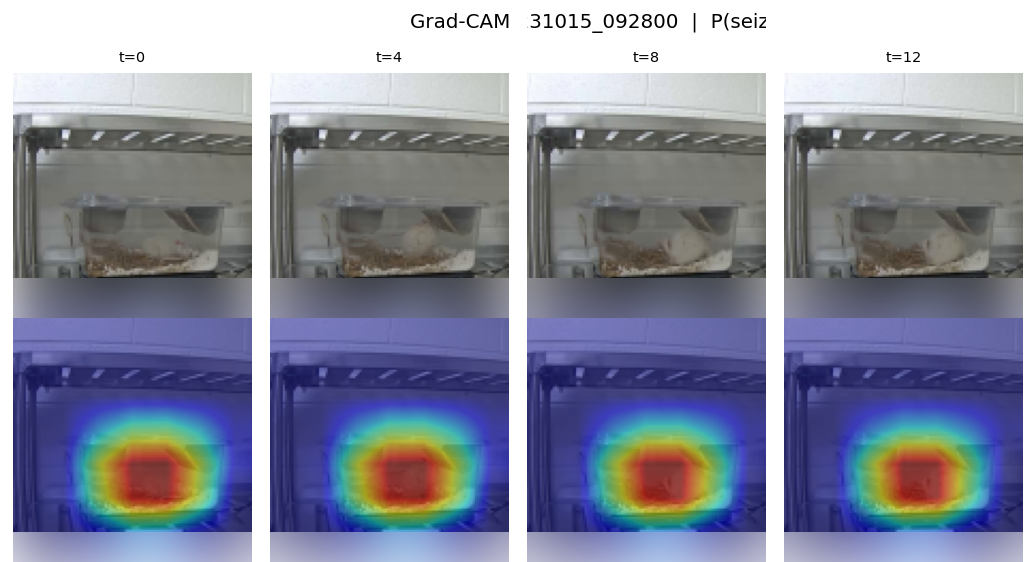
\includegraphics[width=\linewidth, trim=0 0 0 42, clip]{fig/gradcam_stage4_deid_4f.png}\\[1pt]
{\footnotesize (a) Seizure clip (Stage\,4): activation concentrates on the animal}\\[4pt]
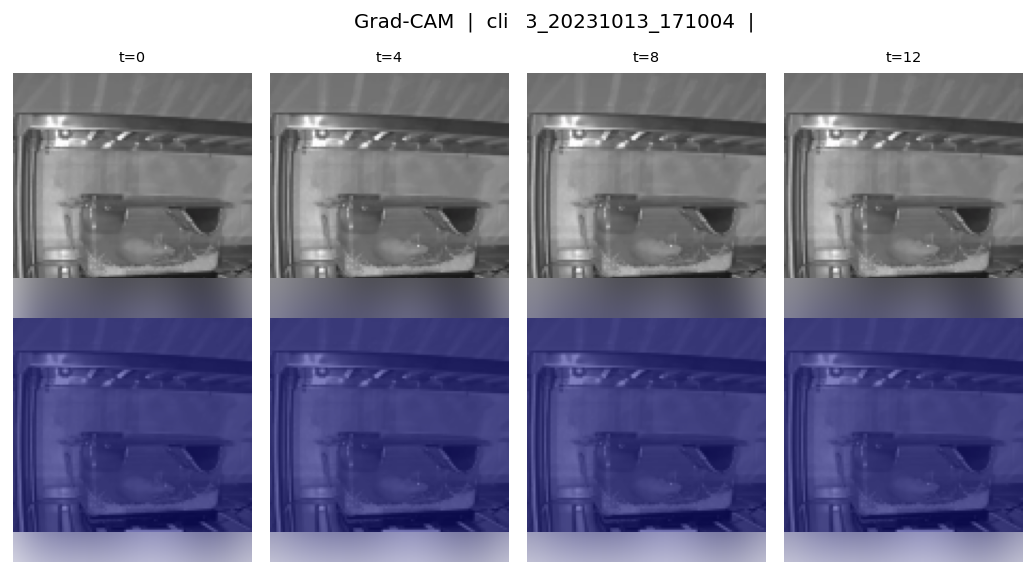
\includegraphics[width=\linewidth, trim=0 0 0 42, clip]{fig/gradcam_nonseizure_deid_4f.png}\\[1pt]
{\footnotesize (b) Non-seizure clip: activation is diffuse, with no focus on the animal}
\caption{Grad-CAM~\cite{selvaraju2017gradcam} for the R(2+1)D detector; each strip
shows input frames (top) and seizure-class activation (bottom), for four of the
eight sampled frames. \emph{(a)}~On a Stage\,4 clip, activation concentrates on the
animal during convulsive motion. \emph{(b)}~On a non-seizure clip it stays diffuse.
The contrast indicates the detector responds to behavior rather than cage
background. All eight frames at full width are in App.~\ref{sec:qualitative:gradcam},
Fig.~\ref{fig:gradcamfull}. De-identified clips; identifier bands redacted.}
\label{fig:gradcam}
\end{figure}



\begin{takeaway}
\takeawaylabel Detection is limited by temporal context rather than by model size. Ten backbones
spanning every paradigm land within 0.03 macro-F1 and a 4M-parameter model ties a 33M
one, while a single frame collapses to 0.569. Sixteen to thirty-two frames at
$112$\,px suffices, and the shortcut controls available to us are consistent with a
behavioral detector without settling the question.
\end{takeaway}

\subsection{Cross-modal comparison, generalization and external validation}
\label{sec:crossmodal}

With the capacity question settled, we turn to how far the video result carries: how
it stands against an electrode-based reference, whether it survives held-out animals
and harder label granularities, and whether it reproduces on a public benchmark.

\noindent\textbf{Is the EEG baseline strong enough?}
Because the headline is a cross-modal comparison, the EEG side must be a strong
baseline. Each EEG model consumes the first recorded EEG channel decimated to
125\,Hz, cut into 6\,s windows at 3\,s stride and z-scored per window; a clip
decision is the log-mean of the per-window posteriors (App.~\ref{sec:eegsweep}). On these identical windows,
split and seed we evaluate seven EEG models (Table~\ref{tab:eegarch}), chosen to
span how the temporal structure of a trace can be modeled. Five are deep. The GRU above and an LSTM~\cite{hochreiter1997lstm} read the window as a raw sequence. EEGNet~\cite{lawhern2018eegnet} is a compact CNN whose first layer acts as a learned bandpass filter bank, the EEG Conformer~\cite{song2022conformer} puts a self-attention encoder over convolutional tokens, and a dilated temporal convolutional network (TCN)~\cite{bai2018tcn} grows its receptive field exponentially with depth. Two are classical: Random Forest~\cite{breiman2001rf} and
XGBoost~\cite{chen2016xgboost} learn no representation and instead consume a fixed
per-window descriptor of band powers and time-domain statistics. The strongest at detection is the TCN, at 0.978\,$\pm$\,0.001 macro-F1 and 0.996
AUROC, a little above the GRU (0.974\,$\pm$\,0.003); it also leads at 3-class
(0.767 \vs\ 0.750). At 5-class the two are tied within seed noise
(0.563\,$\pm$\,0.012 \vs\ 0.560\,$\pm$\,0.005), so the ordering that holds
across the table is TCN\,$\geq$\,GRU\,$>$\,Conformer\,$>$\,LSTM\,$>$\,EEGNet
rather than a single winner. The spread across the five deep models is
0.055 macro-F1 at detection but 0.147 at 3-class and 0.154 at 5-class: architecture
is close to irrelevant for detecting a seizure and matters considerably for grading
one, the mirror image of the backbone-agnostic result on the video side
(Table~\ref{tab:vidarch}). The classical baselines are competitive at detection,
where feature-based XGBoost reaches 0.914 against the deep EEGNet's 0.923, but fall
away at grading (0.466 \vs\ 0.563 for the TCN at 5-class), so the deep advantage on
EEG is small where the task is easy and real where it is hard. The LSTM is the least
reliable model in the field: two of its fifteen runs failed to converge outright,
which no other backbone did. One caveat bounds the absolute margin: this EEG
reference is single-channel, so a richer montage could narrow the reported
cross-modal gap.

Architecture diversity is not tuning, so we also sweep the EEG side's window,
stride, sampling rate and clip-pooling rule, and every model in
Table~\ref{tab:eegarch} is trained at the winning setting
(App.~\ref{sec:eegsweep}). The sweep is informative about which axis matters.
Window length is nearly flat---2, 4, 6 and 8\,s span 0.015 macro-F1, less than the
0.018 range we measure across seeds at a fixed setting---while stride is monotone
(0.554 at 1.5\,s to 0.496 at 6\,s) and sampling rate is the largest single effect
(dropping to 62.5\,Hz costs 0.049). The clip-pooling rule, an axis rarely swept at
all, is worth more than any of them: log-mean beats the usual mean on seven of eight
configurations and gains 0.028 macro-F1 at the winning setting, for free, since it
re-scores stored window posteriors without retraining. Because pooling and window
interact---the best window under mean pooling is only fourth-best under
log-mean---we select the best \emph{pair} rather than optimizing the axes in
sequence. Even so, the tuned EEG reference does not close the cross-modal gap: the
strongest EEG model at 5-class reaches 0.563 against video's 0.657.

\noindent\textbf{Does the ordering depend on the metric?}
Macro-F1 and MCC weight the confusion matrix differently, so we report both
throughout (Sec.~\ref{sec:problem}). They disagree about how hard grading \emph{looks}: at 5-class video scores 0.657 macro-F1 against 0.831 MCC. They agree on every ordering that carries a claim. The cross-modal gap widens with granularity under both, and the ten backbones stay clustered under both. The headline conclusions are therefore a property of the data, not of the summary statistic; App.~\ref{sec:metrics} works this through.

\begin{table*}[t]
\centering
\caption{EEG backbone comparison (identical windows and split) across all three
granularities, as mean\,$\pm$\,std over five seeds. Precision/recall/F1 are
macro-averaged; detection AUROC is binary, grading AUROC macro one-vs-rest; MCC is the
multiclass Matthews correlation coefficient. All models use the configuration selected
in App.~\ref{sec:eegsweep}: 6\,s windows at 3\,s stride, 125\,Hz, logmean clip
pooling. The TCN leads at detection and 3-class; at 5-class it and the GRU are tied
within noise (0.563\,$\pm$\,0.012 \vs\ 0.560\,$\pm$\,0.005). Random Forest and
XGBoost use per-window band-power and time-domain features; XGBoost is deterministic
given the data, hence $\pm$0.000. Two of fifteen LSTM runs failed to converge
(macro-F1 0.231 and 0.136 against cell medians of 0.677 and 0.456); they are excluded
from the LSTM means, which therefore rest on $n{=}3$ at 3-class and $n{=}4$ at 5-class.
Best per column \textbf{bold}, second-best \underline{underlined}.}
\label{tab:eegarch}
\setlength{\tabcolsep}{3pt}
\renewcommand{\arraystretch}{1.15}
\resizebox{\textwidth}{!}{%
\begin{tabular}{@{}l ccccc ccccc ccccc@{}}
\toprule
 & \multicolumn{5}{c}{\textbf{Detection (2-class)}} & \multicolumn{5}{c}{\textbf{3-class}} & \multicolumn{5}{c}{\textbf{5-class}} \\
\cmidrule(lr){2-6}\cmidrule(lr){7-11}\cmidrule(lr){12-16}
\textbf{EEG backbone} & \textbf{P} & \textbf{R} & \textbf{F1} & \textbf{AUC} & \textbf{MCC} & \textbf{P} & \textbf{R} & \textbf{F1} & \textbf{AUC} & \textbf{MCC} & \textbf{P} & \textbf{R} & \textbf{F1} & \textbf{AUC} & \textbf{MCC} \\
\midrule
\multicolumn{16}{@{}l}{\itshape Deep}\\
GRU~\cite{ganguly2025} & \underline{0.975}\,{\scriptsize$\pm$0.003} & \underline{0.974}\,{\scriptsize$\pm$0.003} & \underline{0.974}\,{\scriptsize$\pm$0.003} & \underline{0.996}\,{\scriptsize$\pm$0.001} & \underline{0.949}\,{\scriptsize$\pm$0.005} & \underline{0.744}\,{\scriptsize$\pm$0.014} & 0.764\,{\scriptsize$\pm$0.013} & \underline{0.750}\,{\scriptsize$\pm$0.010} & \underline{0.956}\,{\scriptsize$\pm$0.002} & \underline{0.823}\,{\scriptsize$\pm$0.014} & \textbf{0.556}\,{\scriptsize$\pm$0.040} & \underline{0.635}\,{\scriptsize$\pm$0.035} & \underline{0.560}\,{\scriptsize$\pm$0.005} & \textbf{0.941}\,{\scriptsize$\pm$0.003} & \textbf{0.728}\,{\scriptsize$\pm$0.032} \\
LSTM~\cite{hochreiter1997lstm} & 0.972\,{\scriptsize$\pm$0.008} & 0.971\,{\scriptsize$\pm$0.007} & 0.971\,{\scriptsize$\pm$0.008} & 0.994\,{\scriptsize$\pm$0.004} & 0.942\,{\scriptsize$\pm$0.015} & 0.696\,{\scriptsize$\pm$0.041} & 0.741\,{\scriptsize$\pm$0.067} & 0.698\,{\scriptsize$\pm$0.053} & 0.937\,{\scriptsize$\pm$0.027} & 0.743\,{\scriptsize$\pm$0.059} & 0.476\,{\scriptsize$\pm$0.042} & 0.555\,{\scriptsize$\pm$0.100} & 0.468\,{\scriptsize$\pm$0.052} & 0.903\,{\scriptsize$\pm$0.039} & 0.598\,{\scriptsize$\pm$0.059} \\
EEGNet~\cite{lawhern2018eegnet} & 0.926\,{\scriptsize$\pm$0.011} & 0.922\,{\scriptsize$\pm$0.013} & 0.923\,{\scriptsize$\pm$0.012} & 0.975\,{\scriptsize$\pm$0.005} & 0.848\,{\scriptsize$\pm$0.023} & 0.646\,{\scriptsize$\pm$0.010} & 0.676\,{\scriptsize$\pm$0.018} & 0.620\,{\scriptsize$\pm$0.015} & 0.903\,{\scriptsize$\pm$0.005} & 0.626\,{\scriptsize$\pm$0.031} & 0.448\,{\scriptsize$\pm$0.040} & 0.488\,{\scriptsize$\pm$0.025} & 0.409\,{\scriptsize$\pm$0.039} & 0.864\,{\scriptsize$\pm$0.011} & 0.499\,{\scriptsize$\pm$0.037} \\
EEG Conformer~\cite{song2022conformer} & 0.972\,{\scriptsize$\pm$0.001} & 0.972\,{\scriptsize$\pm$0.001} & 0.972\,{\scriptsize$\pm$0.001} & 0.988\,{\scriptsize$\pm$0.002} & 0.943\,{\scriptsize$\pm$0.001} & 0.719\,{\scriptsize$\pm$0.009} & \underline{0.784}\,{\scriptsize$\pm$0.013} & 0.729\,{\scriptsize$\pm$0.010} & 0.952\,{\scriptsize$\pm$0.002} & 0.780\,{\scriptsize$\pm$0.017} & 0.512\,{\scriptsize$\pm$0.004} & 0.624\,{\scriptsize$\pm$0.032} & 0.523\,{\scriptsize$\pm$0.005} & 0.936\,{\scriptsize$\pm$0.008} & 0.683\,{\scriptsize$\pm$0.008} \\
TCN~\cite{bai2018tcn} & \textbf{0.979}\,{\scriptsize$\pm$0.001} & \textbf{0.978}\,{\scriptsize$\pm$0.001} & \textbf{0.978}\,{\scriptsize$\pm$0.001} & \textbf{0.996}\,{\scriptsize$\pm$0.001} & \textbf{0.957}\,{\scriptsize$\pm$0.002} & \textbf{0.758}\,{\scriptsize$\pm$0.014} & \textbf{0.786}\,{\scriptsize$\pm$0.008} & \textbf{0.767}\,{\scriptsize$\pm$0.007} & \textbf{0.960}\,{\scriptsize$\pm$0.001} & \textbf{0.839}\,{\scriptsize$\pm$0.015} & \underline{0.537}\,{\scriptsize$\pm$0.008} & \textbf{0.654}\,{\scriptsize$\pm$0.013} & \textbf{0.563}\,{\scriptsize$\pm$0.012} & \underline{0.941}\,{\scriptsize$\pm$0.003} & \underline{0.728}\,{\scriptsize$\pm$0.021} \\
\midrule
\multicolumn{16}{@{}l}{\itshape Classical (band-power $+$ statistical features)}\\
Random Forest~\cite{breiman2001rf} & 0.885\,{\scriptsize$\pm$0.001} & 0.852\,{\scriptsize$\pm$0.001} & 0.852\,{\scriptsize$\pm$0.001} & 0.986\,{\scriptsize$\pm$0.000} & 0.737\,{\scriptsize$\pm$0.002} & 0.541\,{\scriptsize$\pm$0.001} & 0.542\,{\scriptsize$\pm$0.001} & 0.529\,{\scriptsize$\pm$0.001} & 0.934\,{\scriptsize$\pm$0.001} & 0.613\,{\scriptsize$\pm$0.002} & 0.477\,{\scriptsize$\pm$0.001} & 0.328\,{\scriptsize$\pm$0.001} & 0.332\,{\scriptsize$\pm$0.002} & 0.916\,{\scriptsize$\pm$0.002} & 0.503\,{\scriptsize$\pm$0.002} \\
XGBoost~\cite{chen2016xgboost} & 0.922\,{\scriptsize$\pm$0.000} & 0.913\,{\scriptsize$\pm$0.000} & 0.914\,{\scriptsize$\pm$0.000} & 0.984\,{\scriptsize$\pm$0.000} & 0.835\,{\scriptsize$\pm$0.000} & 0.657\,{\scriptsize$\pm$0.000} & 0.684\,{\scriptsize$\pm$0.000} & 0.642\,{\scriptsize$\pm$0.000} & 0.934\,{\scriptsize$\pm$0.000} & 0.623\,{\scriptsize$\pm$0.000} & 0.479\,{\scriptsize$\pm$0.000} & 0.530\,{\scriptsize$\pm$0.000} & 0.466\,{\scriptsize$\pm$0.000} & 0.924\,{\scriptsize$\pm$0.000} & 0.529\,{\scriptsize$\pm$0.000} \\
\bottomrule
\end{tabular}}
\end{table*}

\noindent\textbf{Generalization to unseen subjects.}
Session-disjoint validation still trains and tests on the \emph{same} animals. The
stricter, deployment-relevant question is whether the detector transfers to an animal it has never seen, the protocol RodEpil~\cite{rodepil2025} adopts. We
therefore repeat all three tasks under \emph{subject-disjoint} five-fold
cross-validation, holding out four whole animals per fold
(Table~\ref{tab:subjectwise}). At detection, neither modality is much troubled by the
harder protocol. Video degrades only marginally, from 0.968 to 0.948 macro-F1 and 0.993 to 0.985 AUROC. The EEG GRU is essentially unchanged, moving from 0.974 to 0.972, and the two fold spreads are nearly identical ($\sigma$ 0.016 against 0.019). The two are therefore equally stable across held-out animals, and EEG ends up marginally ahead. That reverses the session-disjoint ordering, though both differences are small relative to the fold spread (Fig.~\ref{fig:stability}). Detection generalizes across animals in both
modalities; the modalities separate at grading, not here. Part of the residual
cross-subject difficulty is visual: cage framing, lighting, and coat vary from
animal to animal (App.~\ref{sec:dataextra:crosssubj}, Fig.~\ref{fig:crosssubj}).

Grading is where the protocol bites. Holding out whole animals costs video 0.060
macro-F1 at 3-class and 0.182 at 5-class (0.780\,$\to$\,0.720 and
0.657\,$\to$\,0.475), against 0.094 and 0.156 for the EEG reference, so the cross-modal margin at 5-class narrows from 0.097 to 0.071. Video still leads at both grading granularities: 0.720 against 0.656 at 3-class, and 0.475 against 0.404 at 5-class. The two now degrade at comparable rates, and video is no longer uniformly the steadier across folds.
We read the larger video drop as the price of appearance: a held-out animal arrives
with unfamiliar cage framing, lighting and coat, and at five classes the model must
separate stages that differ by subtle motion on top of that shift. Fine-grained
grading across unseen animals is thus the weakest regime we measure for either
modality, and the accurate statement of our result is that video's advantage is
largest within a cohort and narrower, though still substantial, across new animals.

% fig:crosssubj now lives in the supplement (App. C, sec:dataextra:crosssubj).


\begin{figure}[t]
\centering
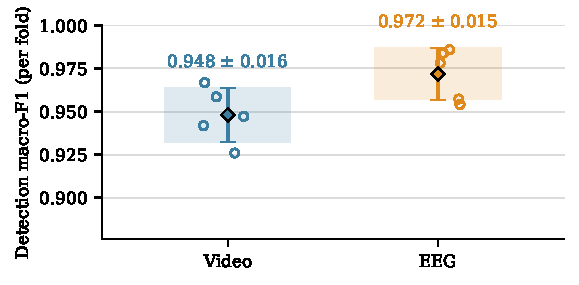
\includegraphics[width=\linewidth]{fig/fig_stability.pdf}
\caption{Cross-subject stability under subject-disjoint 5-fold CV (per-fold
detection macro-F1 from Table~\ref{tab:subjectwise}; dots are folds, diamonds are
the mean, whiskers/bands are $\pm1\sigma$). Both modalities are tightly and comparably clustered, video at $0.948\pm0.016$ over $[0.926,0.967]$ and EEG at $0.972\pm0.015$ over $[0.954,0.986]$, so detection transfers to unseen animals about equally well either way, with EEG marginally ahead on the mean. The
modalities diverge at grading instead (Table~\ref{tab:subjectwise}).}
\label{fig:stability}
\end{figure}

\begin{table}[tb]
\centering
\caption{Generalization from session-disjoint to subject-disjoint (5-fold, whole animals
held out) at all three granularities. The protocols separate the two regimes cleanly.
At detection, holding out whole animals costs video 0.022 macro-F1 and costs the EEG reference nothing (0.974\,$\to$\,0.972), so EEG is ahead on unseen animals and the two
are equally stable across folds ($\pm$0.015 \vs\ $\pm$0.016; MCC $\pm$0.030 \vs\
$\pm$0.031). At grading video leads under both protocols, though it gives up more when animals are held out, 0.187 macro-F1 at 5-class against 0.159 for EEG, so the margin narrows from 0.128 to 0.100. Subject-disjoint entries are mean\,$\pm$\,std over folds.}
\label{tab:subjectwise}
\setlength{\tabcolsep}{3pt}
\renewcommand{\arraystretch}{1.2}
\resizebox{\columnwidth}{!}{%
\begin{tabular}{@{}l l cc ccc@{}}
\toprule
 & & \multicolumn{2}{c}{\textbf{Session-dis.}} & \multicolumn{3}{c}{\textbf{Subject-disjoint (5-fold)}} \\
\cmidrule(lr){3-4}\cmidrule(lr){5-7}
\textbf{Task} & \textbf{Mod.} & \textbf{Macro-F1} & \textbf{MCC} & \textbf{Macro-F1} & \textbf{AUROC} & \textbf{MCC} \\
\midrule
\multirow{2}{*}{Detection} & Video & 0.968 & 0.936 & 0.948\,{\scriptsize$\pm$0.016} & 0.985\,{\scriptsize$\pm$0.006} & 0.896\,{\scriptsize$\pm$0.031} \\
                           & EEG   & \textbf{0.974} & \textbf{0.949} & \textbf{0.972}\,{\scriptsize$\pm$0.015} & \textbf{0.995}\,{\scriptsize$\pm$0.005} & \textbf{0.944}\,{\scriptsize$\pm$0.030} \\
\midrule
\multirow{2}{*}{3-class}   & Video & \textbf{0.780} & \textbf{0.853} & \textbf{0.720}\,{\scriptsize$\pm$0.028} & \textbf{0.942}\,{\scriptsize$\pm$0.015} & 0.761\,{\scriptsize$\pm$0.029} \\
                           & EEG   & 0.750 & 0.823 & 0.656\,{\scriptsize$\pm$0.022} & 0.916\,{\scriptsize$\pm$0.025} & \textbf{0.793}\,{\scriptsize$\pm$0.046} \\
\midrule
\multirow{2}{*}{5-class}   & Video & \textbf{0.657} & \textbf{0.831} & \textbf{0.475}\,{\scriptsize$\pm$0.024} & \textbf{0.888}\,{\scriptsize$\pm$0.026} & \textbf{0.676}\,{\scriptsize$\pm$0.041} \\
                           & EEG   & 0.560 & 0.728 & 0.404\,{\scriptsize$\pm$0.042} & 0.831\,{\scriptsize$\pm$0.076} & 0.657\,{\scriptsize$\pm$0.107} \\
\bottomrule
\end{tabular}}
\end{table}

\noindent\textbf{Grading: video degrades, EEG collapses.}
Severity is harder, and here the two modalities part ways. As the task moves from
2-class detection to 3-class (non-seizure / mild / severe) and 5-class
(non-seizure / Stage\,2--5) grading, video macro-F1 declines gracefully from
0.968 to 0.780 to 0.657 and stays usable even at five levels. Even the rare severe
classes retain a workable signal (Stage\,5 per-class F1 0.42 at 5-class;
App.~\ref{sec:extraresults:ablations}, Table~\ref{tab:perclass}). The EEG reference
declines more steeply from the same starting point
(0.974\,$\to$\,0.750\,$\to$\,0.560), and its rarest classes are where it gives way
(Stage\,4 F1 0.20, Stage\,5 F1 0.12 against 0.36 and above for video; the per-class
breakdown is given in Table~\ref{tab:perclass} and Figure~\ref{fig:perclassbar}).
Video thus retains a workable severity signal where EEG does not, though
fine-grained grading remains the weakest regime for both. The hardest cases are
rare mild events and data-poor animals (App.~\ref{sec:qualitative:failures},
Fig.~\ref{fig:hardcases}). Figure~\ref{fig:degrade} traces the two
curves side by side: they start level but the video line stays high while the EEG
line dives, the gap widening from 0.004 at detection to 0.128 at 5-class.

\noindent\textbf{Do the two modalities fail the same way?}
An aggregate gap says which model is better, not whether the other is redundant, so
we compare the errors themselves (App.~\ref{sec:extraresults:failure},
Fig.~\ref{fig:confusion}). They differ in kind. Video's mistakes are ordinal
near-misses: $72.4\%$ land on an adjacent stage, and the largest single cell is
Stage\,4 read as Stage\,3 ($95$ of $167$ clips). It registers that a convulsion is
underway and misjudges the degree. The EEG reference adds two failure modes video
does not have. It loses events outright, calling $10.1\%$ of Stage\,3 clips non-seizure against $2.3\%$ for video, and its errors ignore the ordinal scale,
$44\%$ landing two or more stages away against $28\%$ for video (mean
$|\Delta\text{stage}|$ $1.51$ \vs\ $1.30$). A single channel supports a
seizure/no-seizure decision without carrying a monotone severity axis. The one
exception is the informative one: at Stage\,2, the rung with the least whole-body
movement, the ordering reverses and EEG recalls $0.863$ against video's $0.650$.
Video's advantage is behavioral, and it recedes exactly where the behavior does.
Across the clips both models scored, video alone is correct on $14.2\%$ and EEG
alone on $4.9\%$ (Table~\ref{tab:paired}), so each modality recovers clips the other
loses. That is a measured case for the fusion we leave to future work
(Sec.~\ref{sec:open}).

% fig:hardcases now lives in the supplement (App. D, sec:qualitative:failures).

\begin{figure}[t]
\centering
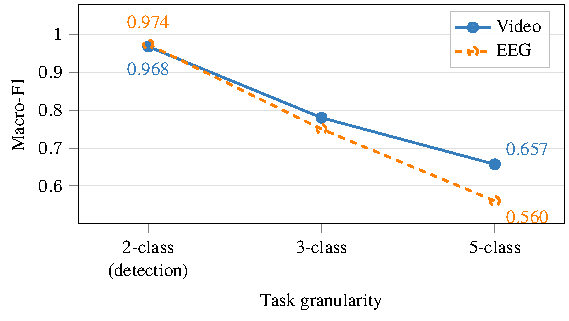
\includegraphics[width=\linewidth]{fig/fig_degrade.pdf}
\caption{Video degrades more gracefully than EEG as the task hardens (macro-F1,
values from Table~\ref{tab:results}). The two modalities are level at detection
(0.968 \vs\ 0.974), and by 5-class grading video still retains a usable 0.657
whereas the EEG GRU falls to 0.560, so a 0.006 EEG lead at detection becomes a 0.097 video lead at five classes.}
\label{fig:degrade}
\end{figure}

\noindent\textbf{External validation on RodEpil.}
To test whether these detection numbers transfer beyond our own cohort, we
evaluate the same R(2+1)D backbone on the public RodEpil
benchmark~\cite{rodepil2025} (13{,}053 clips, 19 rats) under its native
\emph{subject-wise} five-fold protocol. A direct run scores a suspicious 0.9996
F1, because the raw release leaks the class label into low-level clip encoding.
Every normal clip is stored at 30\,fps / 301 frames and every seizure clip at
29\,fps / 291 frames. Either attribute alone separates the classes with AUROC 1.0, and the per-clip crop resolution also differs by class. Re-encoding
all clips through a single uniform pipeline ($224\times224$ letterbox, 30\,fps,
300 frames, identical codec) removes this shortcut, and the backbone then reaches
\textbf{0.979 subject-wise F1} (AUROC 0.999; per-fold in Table~\ref{tab:rodepil}).
This matches the dataset's TimeSformer baseline (0.97) and reflects genuine
behavior: the per-fold learning curve now rises gradually instead of saturating
at epoch one. We flag the encoding confound as a caution for future users of this
otherwise valuable benchmark.

\begin{table}[tb]
\centering
\caption{External validation on RodEpil~\cite{rodepil2025} (subject-wise 5-fold,
seizure-class F1 and MCC). The raw release is separable by an encoding artifact that
inflates detection to near-perfect; re-encoding every clip through one uniform
pipeline removes the shortcut and yields honest scores on par with the dataset's
TimeSformer baseline (0.97).}
\label{tab:rodepil}
\setlength{\tabcolsep}{5pt}
\renewcommand{\arraystretch}{1.15}
\resizebox{\columnwidth}{!}{%
\begin{tabular}{@{}l ccccc c@{}}
\toprule
 & \textbf{F0} & \textbf{F1} & \textbf{F2} & \textbf{F3} & \textbf{F4} & \textbf{Mean} \\
\midrule
Raw (leaked) F1  & 1.000 & 0.998 & 1.000 & 1.000 & 1.000 & \textbf{0.9996} \\
Raw (leaked) MCC & 1.000 & 0.998 & 1.000 & 1.000 & 1.000 & \textbf{0.9995} \\
\midrule
Re-encoded F1    & 0.965 & 0.978 & 0.997 & 0.977 & 0.979 & \textbf{0.979} \\
Re-encoded AUROC & 0.999 & 1.000 & 1.000 & 1.000 & 0.998 & \textbf{0.999} \\
Re-encoded MCC   & 0.957 & 0.976 & 0.996 & 0.967 & 0.964 & \textbf{0.972} \\
\bottomrule
\end{tabular}}
\end{table}

\noindent\textbf{All backbones on RodEpil.}
Running the full ten-backbone suite on re-encoded RodEpil reshuffles the ranking and widens it, from a 0.03 band on our own cohort to 0.87--0.99 macro-F1. The convolutional networks lead and the attention models trail, the reverse of our ordering. Backbone choice is therefore a data-regime effect, not a universal ranking (App.~\ref{sec:extraresults}, Table~\ref{tab:rodepilbb}).

\begin{figure}[t]
\centering
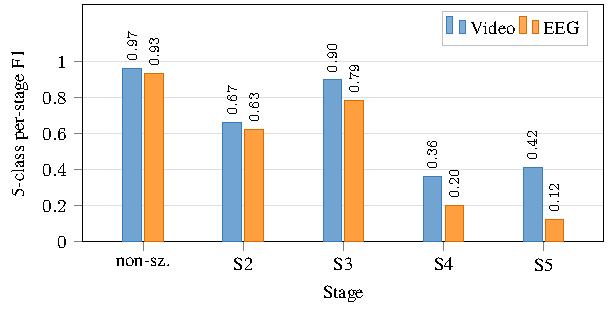
\includegraphics[width=\linewidth]{fig/fig_perclassbar.pdf}
\caption{Per-stage F1 at the hardest 5-class grading task
(Table~\ref{tab:perclass}). Both modalities are strong on the common classes, non-seizure and Stage\,3. On the rare severe stages EEG gives way, with S4/S5 F1 of 0.20 and 0.12, while video retains a usable signal at 0.36 and 0.42. Video holds a workable severity cue where the electrode-based model gives out.}
\label{fig:perclassbar}
\end{figure}



\begin{takeaway}
\takeawaylabel Video matches the EEG reference at detection (0.968 against 0.974)
and pulls ahead as the task becomes behavioral, reaching 0.657 against 0.560 at five-class. That ordering survives both held-out animals and the public RodEpil benchmark, though the margin is widest within a cohort and narrows once whole animals are held out. The two also fail differently: video misgrades by one stage, EEG loses events and scatters across non-adjacent ones, and at Stage\,2 the ordering reverses. Their errors are complementary.
\end{takeaway}

\subsection{Does inverse-frequency weighting keep the long tail from
dominating the result?}
\label{sec:rq3}

Two independent imbalances run through this cohort, and both threaten to turn a
pooled score into a report on the majority. The first is across stages: the
five-class validation set is $51\%$ non-seizure and $41\%$ Stage\,3, while Stage\,5
is 34 clips, a ratio of $80{:}1$ between the largest and smallest class. The second
is across animals, whose totals span 11 to 3{,}091 clips
(App.~\ref{sec:dataextra:cohort}). A model that ignored every rare stage and every
quiet animal could still look strong on aggregate accuracy.

\noindent\textbf{Three defenses, at construction, objective and measurement.}
Detection sidesteps the problem by construction: each seizure clip is paired with a
matched negative, so the binary task is near-balanced ($12{,}197$ against
$11{,}934$) and imbalance enters only at grading. At grading the objective carries
it: we train with inverse-frequency-weighted cross-entropy, weights normalized to
mean one, which at five-class gives Stage\,5 roughly $60\times$ the weight of
non-seizure. Measurement then keeps the tail visible. Every score is macro-averaged, every pooled number is paired with a per-subject breakdown, and the generalization study holds out whole animals (Table~\ref{tab:subjectwise}). A model that quietly abandons the tail cannot hide behind a pooled figure. One caveat applies to the metrics themselves. AUROC is optimistic under strong imbalance~\cite{saito2015prc}, which is why macro-F1 carries the argument at the rare stages.

\noindent\textbf{The tail stays learnable.}
The defenses work in the sense that matters first: the rare stages are predicted
rather than weighted out of existence. A majority-class predictor reaches only
0.136 macro-F1 at five-class, against the video model's 0.657, and the model still
recovers a third of the Stage\,5 clips (recall 0.324 on 34 examples) at 0.579
precision (Table~\ref{tab:perclass}).

\noindent\textbf{What it costs.}
Re-weighting redistributes error rather than removing it, and two limits follow.
The tail remains the weakest regime: Stage\,4 and Stage\,5 F1, 0.362 and 0.415, sit far below Stage\,3 at 0.900. The correction mitigates imbalance without solving it. More
instructive is what happens when the same correction meets a weaker signal. The EEG
model's Stage\,5 precision is 0.014 against recall 0.121: it assigns Stage\,5 to
roughly nine times as many clips as actually carry it, converting a rare-class blind
spot into a false-positive one. Up-weighting a class the modality cannot separate buys recall at a price in precision that a screening tool would not accept. The imbalance strategy should therefore be chosen per modality, not globally.

One caveat bounds all of this. We report the behavior of a single reasonable strategy: inverse-frequency weighting is never compared against unweighted training, resampling~\cite{chawla2002smote} or a focal objective~\cite{lin2017focal}, three standard options surveyed in~\cite{johnson2019imbalance} (Sec.~\ref{sec:open}).

\begin{takeaway}
\takeawaylabel Weighting keeps the tail learnable rather than solving it. Rare stages are
predicted instead of collapsing to the majority (0.657 macro-F1 against 0.136 for a
majority-class predictor, with Stage\,5 recall 0.324 on 34 clips), yet they remain
the weakest regime, and on the weaker modality the same correction over-predicts
Stage\,5 roughly ninefold.
\end{takeaway}

\subsection{Why behavioral video matters}
\label{sec:discussion}

Taken together, the results show a camera matching electrodes at detection under
both protocols and pulling ahead once the endpoint is itself behavioral. Three
consequences follow.

\noindent\textbf{Video reads the endpoint directly.}
The Racine scale grades motor manifestations: twitching, rearing, forelimb clonus,
falling~\cite{racine1972}. A camera observes the signal the grade is defined on,
while an electrode observes a correlate of it. That is the simplest account of
Fig.~\ref{fig:degrade}. The modalities are indistinguishable while the question is
whether an event occurred, and separate once it becomes how severe that event was,
with the largest gap at the rarest and most severe stage (Stage\,5 per-class F1
0.42 against 0.12).

\noindent\textbf{Cost, scale and welfare favor the camera.}
Electrode EEG needs surgical implantation, which is expensive, low-throughput, and a
source of infection, signal drift and welfare burden. A camera is cheap,
surgery-free, and watches many cages at once, so video-only screening scales to the
cohorts preclinical drug discovery needs and reduces harm in the spirit of the 3Rs.
Deployment is equally favorable: the 4M-parameter X3D-M matches the 33M R(2+1)D
(Table~\ref{tab:vidspec}), which puts continuous monitoring on modest hardware
within reach.

\noindent\textbf{Electrodes remain necessary, and fusion is the next step.}
Our EEG reference is a single channel, and its limits show throughout: it loses
$10.1\%$ of Stage\,3 events outright, carries no monotone severity axis, and
supplies no localization. A richer montage would ease all three. Even so, EEG
captures electrographic-only seizures that have no motor correlate at all, recovers
onset timing, and recovers the Stage\,2 events video misses
(Sec.~\ref{sec:crossmodal}); a camera is blind to each of these. Video does not
displace the electrode; it carries the behavioral half of the workflow, which is the
half that consumes expert time. We keep the two streams unfused here deliberately.
A fused model would confound the question we set out to answer, namely how far each modality gets on its own. No shared paired video--EEG benchmark yet exists on which such a model could be compared against prior work (Sec.~\ref{sec:open}).

\begin{takeaway}
\takeawaylabel A camera alone matches electrode-based detection, on held-out
sessions and held-out animals alike, and grades severity more accurately.
Electrodes stay necessary for electrographic-only events, onset timing, and the
mildest behavioral stage.
\end{takeaway}

